\documentclass{report}
\usepackage[margin=1in, paperwidth=8.5in, paperheight=11in]{geometry}
%Math packages%
\usepackage{amsmath}
\usepackage{amsthm}
%Spacing%
\usepackage{setspace}
\onehalfspacing
%Lecture number%
\newcommand{\lectureNum}{1}
%Variables - Date and Course%
\newcommand{\curDate}{January 4, 2017}
\newcommand{\course}{MATH 239}
\newcommand{\instructor}{Luke Postle}
%Defining the example tag%
%\theoremstyle{definition}%
\newtheorem{ex}{Example}[section]
%Setting counter given the lecture number%
\setcounter{chapter}{\lectureNum{}}
%Package for drawing graphs%
\usepackage{tikz}
\usepackage{verbatim}
\usetikzlibrary{arrows}

\begin{document}
%Note title%
\begin{center}
\begin{Large}
\textsc{\course{} | Lecture \lectureNum{}}
\end{Large}
\end{center} 
\noindent \textit{Bartosz Antczak} \hfill
\textit{Instructor: \instructor{}} \hfill
\textit{\curDate{}}
\rule{\textwidth}{0.4pt}
% Actual Notes%
\section{Course Info}
Combinatorics began growing in the fifties and sixties. Some of its progressive development was thanks to some professors here at Waterloo! \\
This course will cover two major topics (first half before reading week, second half after reading week):
\begin{itemize}
\item Graph theory (structure of networks, trees, planarity, matching)
\item Enumerative combinatorics (counting, generating series)
\end{itemize}
We will study these topics, but what will we \textit{learn}?
\begin{itemize}
\item new terminology and concepts
\item to prove combinatorially (that's what math is: logic and proofs)
\item new proof techniques/tricks
\item to THINK (combinatorially)
\end{itemize}

\section{Graph Theory | Introduction}
Let's start with a definition, what is a \textit{graph}? In combinatorics, a \textbf{graph} is a set of elements called \underline{vertices} (or nodes in CS) and a set of pairs of distinct vertices called \underline{edges}.
\subsubsection{Notation}
If $G$ is a graph, we let $V(G)$ denote the set of vertices and $E(G)$  denote the set of edges. For instance, consider graph $G$ with one vertex called $a$: $V(G) = \{a\}$, $E(G) = \emptyset$ \\
We can also \textit{draw} graphs, where vertices are points and edges are lines/curves connecting the pairs of vertices. We will tend to drawing graphs rather than using the previous notation.

%EXAMPLE 1%
\begin{ex}
Let's draw the graph described by $V = \{x, y, z\}$, $E = \{xy, yz\}$ \\
\end{ex}
%Graph 1%
\begin{center}
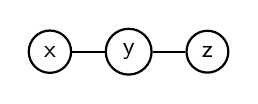
\begin{tikzpicture}[-,auto,node distance=1cm,
                    thick,main node/.style={circle,draw,font=\sffamily\small}]

  \node[main node] (1) {z};
  \node[main node] (2) [left of=1] {y};
  \node[main node] (3) [left of=2] {x};

  \path[every node/.style={font=\sffamily\small}]
    (1) edge node [left] {} (2)
    (2) edge node [left] {} (3);
\end{tikzpicture}
\end{center}

%EXAMPLE 2%
\begin{ex}
A disconnected graph (it appears to look like two graphs, but it's actually one). Defined by $V = \{1, 2, 3, 4, 5\}$, $E = \{12,\, 34,\, 35,\, 45\}$. We'll cover this more next week.
\end{ex}
%Graph 2%
\begin{center}
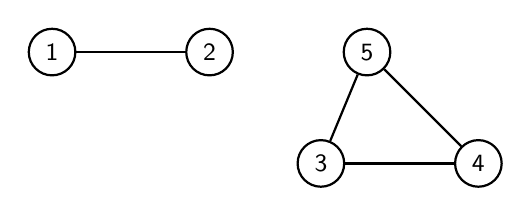
\begin{tikzpicture}[-,auto,node distance=2cm,
                    thick,main node/.style={circle,draw,font=\sffamily\small}]

  \node[main node] (1) {1};
  \node[main node] (2) [right of=1] {2};
  \node[main node] (3) [below right of=2] {3};
  \node[main node] (4) [right of=3] {4};
  \node[main node] (5) [above left of=4] {5};
    
  \path[every node/.style={font=\sffamily\small}]
    (1) edge node [left] {} (2)
    (3) edge node [left] {} (4)
    (3) edge node [left] {} (5)
    (5) edge node [right] {} (4);
\end{tikzpicture}
\end{center}


\subsubsection{More examples of graphs}

%Graph 3 - K_n series%
\begin{ex}
$K_n$ denotes the \underline{complete graph} on $n$ vertices, where ``complete" means that all pairs of vertices are edges (one vertex is connected to every other vertex). This is our first graph \textbf{family}.\\The graphs $K_3$ and $K_4$ are shown below:
\end{ex}
%Graph 3%
\begin{center}
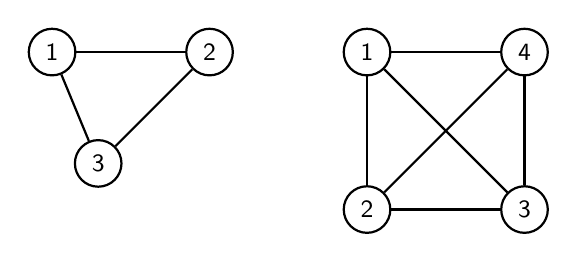
\begin{tikzpicture}[-,auto,node distance=2cm,
                    thick,main node/.style={circle, draw,font=\sffamily\small}]

  %Triangle%
  \node[main node] (1) {1};
  \node[main node] (2) [right of=1] {2};
  \node[main node] (3) [below left of=2] {3};
  %Square%
  \node[main node] (4) [right of=2]{1};
  \node[main node] (5) [below of=4]{2};
  \node[main node] (6) [right of=5]{3};
  \node[main node] (7) [above of=6]{4};
  
  \path[every node/.style={font=\sffamily\small}]
    (1) edge node [left] {} (2)
    (1) edge node [left] {} (3)
    (2) edge node [right] {} (3)
    
    %Square%
    (4) edge node [right] {} (7)
        edge node [right] {} (5)
        edge node [right] {} (6)
    (6) edge node [right] {} (5)
        edge node [right] {} (7)
    (5) edge node [right] {} (7);
\end{tikzpicture}
\end{center}

%EXAMPLE 4%
\begin{ex}
$C_n$ denotes the cycle on $n$ vertices. More formally, if $V = \{v_1, v_2, \cdots, v_n\}$, then $E = \{v_1v_2,\, v_2v_3,\, \cdots, \,v_{n-1}v_{n},\, v_nv_1\}$. $C_5$ is shown:
\end{ex}

%Graph 4%
\begin{center}
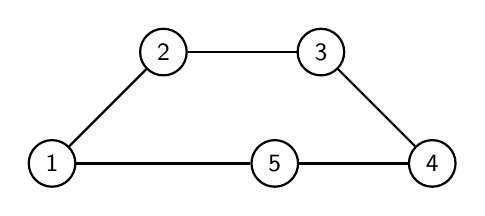
\begin{tikzpicture}[-,auto,node distance=2cm,
                    thick,main node/.style={circle, draw,font=\sffamily\small}]

  %Triangle%
  \node[main node] (1) {1};
  \node[main node] (2)[above right of=1] {2};
  \node[main node] (3)[right of=2] {3};
  \node[main node] (4)[below right of=3] {4};  
  \node[main node] (5)[left of=4] {5};
  
  \path[every node/.style={font=\sffamily\small}]
    (1) edge node [left] {} (2)
        edge node [right] {} (5)
    (2) edge node [left] {} (3)
    (3) edge node [right] {} (4)
    (4) edge node [right] {} (5);
\end{tikzpicture}
\end{center}

%EXAMPLE 5%
\begin{ex}
$P_n$ denotes the path on $n$ vertices, similar to $C_n$ but there is no cycle. If $V = \{v_1, v_2, \cdots, v_n\}$, then $E = \{v_1v_2,\, v_2v_3, \cdots,\, v_{n-1}v_{n}\}$. $P_3$ is shown:
\end{ex}

%Graph 5%
\begin{center}
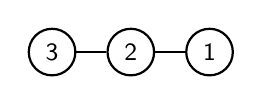
\begin{tikzpicture}[-,auto,node distance=1cm,
                    thick,main node/.style={circle,draw,font=\sffamily\small}]

  \node[main node] (1) {1};
  \node[main node] (2) [left of=1] {2};
  \node[main node] (3) [left of=2] {3};

  \path[every node/.style={font=\sffamily\small}]
    (1) edge node [left] {} (2)
    (2) edge node [left] {} (3);
\end{tikzpicture}
\end{center}

%EXAMPLE 6%
\begin{ex}
$K_{m, n}$ denotes the complete bipartite graph on $m$ and $n$ vertices.\\
$V(K_{m,\,n}) = \{x_1, \cdots, \, x_m, \, y_1, \cdots, \, y_n\}$ with $E = \{x_i\,y_j : \forall \,i, j \;\vert \; 1 \leq i \leq m, \, 1 \leq j \leq n \}$. $K_{2, 3}$ is shown:
\end{ex}

%Graph 6%
\begin{center}
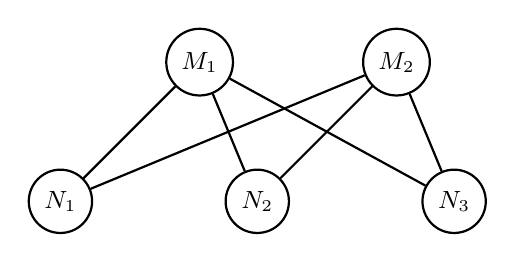
\begin{tikzpicture}[-,auto,node distance=2.5
cm,
                    thick,main node/.style={circle,draw,font=\sffamily\small}]

  %M%
  \node[main node] (1) {$M_1$};
  \node[main node] (2) [right of=1] {$M_2$};
  %N%
  \node[main node] (3) [below left of=1] {$N_1$};
  \node[main node] (4) [right of=3] {$N_2$};
  \node[main node] (5) [right of=4] {$N_3$};

  \path[every node/.style={font=\sffamily\small}]
    (1) edge node [left] {} (3)
    	edge node [left] {} (4)
    	edge node [left] {} (5)
    (2) edge node [left] {} (3)
       	edge node [left] {} (4)
	    edge node [left] {} (5);
\end{tikzpicture}
\end{center}

%Midterm Thursday, March 2, 2017, entirely on graph theory%
%END%
\end{document}